\chapter{Desenvolvimento do sistema}

O principal objetivo do projeto é o de controlar a indução magnética gerada em uma região especifica. A bobina de Helmholtz 3D é capaz de gerar um campo constante e homogêneo no centro de sua estrutura podendo ser controlada por corrente elétrica.

O digrama mostrado na figura \ref{fig:diag2} representa um sistema que utiliza diversas ferramentas para gerar as correntes na bobina de Helmholtz 3D. Um microcontrolador (MCU) verifica o campo gerado pelas bobinas através de um sensor magnético posicionado no centro das estruturas. O MCU se comunica com um computador, recebendo comando de controle das Pontes H que controlam as polaridades das correntes nas bobinas e também enviando os valores de campos lidos pelo sensor.

\begin{figure}[H]
    \centering
     \caption{Diagrama de blocos do sistema.}
     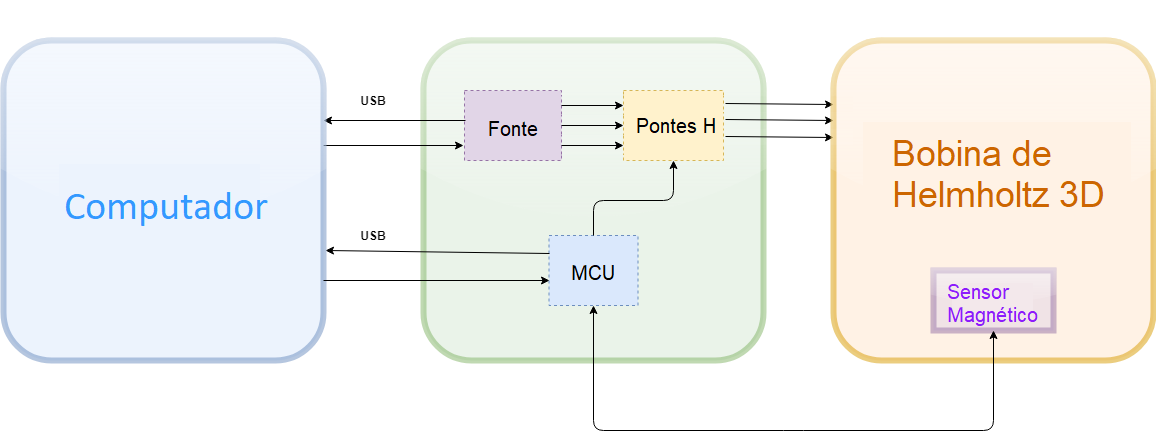
\includegraphics[width=1\textwidth]{./img/diagramas/Blocks diagram 2.png}
     \caption*{Fonte: Autor.}
     \label{fig:diag2}
\end{figure}

\section{Controle das bobinas}

\subsection{Fonte}

A fonte RIGOL 831-A \cite{RG831A} foi escolhida para a alimentação das bobinas de helmholtz. Contém 3 canais, um para cada bobina de Helmholtz a ser controlada, com o canal 3 de tensão negativa e referencia compartilhada com o canal 2. Segundo a folha de dados, a fonte tem resolução de corrente de 100 $\mu$A \cite{RG831A} e pode ser programada por VISA. Uma imagem ilustrativa pode ser vista na figura \ref{fig:font}.

\begin{figure}[H]
    \centering
     \caption{Fonte escolhida para o projeto.}
     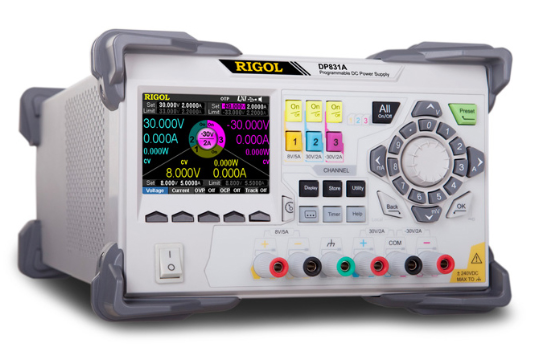
\includegraphics[width=0.8\textwidth]{./img/bob/fonte.png}
     \caption*{Fonte: Folha de dados Rigol DP831A.}
     \label{fig:font}
\end{figure}

\subsection{Ponte H}

Para este projeto foram necessárias 3 pontes H, uma para cada bobina Helmholtz que compõe a bobina de Helmholtz 3D. Ainda há a peculiaridade do canal com tensão negativa o qual a referencia está intrinsecamente conectada a outro canal positivo da fonte do projeto. Isso pode ocasionar um problema de detecção do sinal controle enviado pelo microcontrolador devido a referência da ponte H para o canal negativo estar conectada a uma tensão negativa e a do microcontrolador na referencia do circuito.

Para os canais positivos o CI (Circuito integrado) selecionado foi o DRV8838 \cite{drv8838}, esse é um CI  dedicado, que pode ser controlado com apenas 1 pino digital. A figura \ref{fig:pontHCI} ilustra um diagrama simplificado do DRV8838.

\begin{figure}[H]
    \centering
     \caption{Diagrama simplificado DRV8838.}
     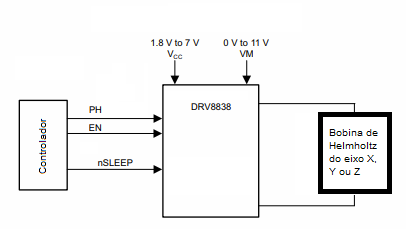
\includegraphics[width=0.8\textwidth]{./img/imagensExplicacoes/ponteHCI.png}
     \caption*{Fonte: Folha de dados DRV8838DSGR.\cite{drv8838}}
     \label{fig:pontHCI}
\end{figure}

Para garantir o funcionamento da ponte H no canal negativo optou-se por utilizar uma ponte H clássica \cite{ponteH} utilizando relés de estado sólido, que são transistores ativados por luz. Estes relés isolam eletricamente o MCU e a ponte H, fazendo com que o sinal de controle do microcontrolador seja detectado independente das referencias utilizadas no circuito da ponte H. Na figura \ref{fig:pontHOpt} é ilustrado o diagrama do componente utilizado para esse propósito.

\begin{figure}[H]
    \centering
     \caption{Diagrama do CPC1002N.}
     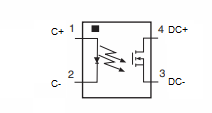
\includegraphics[width=0.5\textwidth]{./img/imagensExplicacoes/ponteHOpt.png}
     \caption*{Fonte: Folha de dados CPC1002N.}
     \label{fig:pontHOpt}
\end{figure}

No diagrama da figura \ref{fig:pontH} pode-se ver o esquemático da ponte H formada pela interligação desses relés, S1 e S4 funcionam juntos, assim como S2 e S3. Os dois conjuntos funcionam alternadamente, ou seja, se as chaves S1 e S4 foram ativadas, S2 e S3 serão desativadas, fazendo o sentido da corrente na carga circular da esquerda para a direita. Se as chaves S2 e S3 forem ativadas, S1 e S4 serão desativadas, fazendo com que a corrente na carga circule da direita para a esquerda.

\begin{figure}[H]
    \centering
     \caption{Ponte H isoladora.}
     \includegraphics[width=0.75\textwidth]{./img/imagensExplicacoes/ponte_h_rele.png}
     \caption*{Fonte: Autor.}
     \label{fig:pontH}
\end{figure}

A escolha dos componentes foi feita pela capacidade de corrente dos componentes que é maior que 500 mA. Essa é a corrente máxima escolhida para circular em cada bobina de Helmholtz e sera discutido na seção 3.3.

\subsection{Microcontrolador}

Era necessário que o microcontrolador tivesse um barramento I2C, 6 pinos de entrada/saída digital para o controle das pontes H e alguma forma de comunicação com o computador, sendo preferível a USB.

Com base nos parametros supracitados, o microcontrolador escolhido para o projeto foi o STM32L432, que emprega a arquitetura ARM Cortex-M4, com ponto flutuante em hardware. Dessa forma, empregou-se o kit de desenvolvimento STM32L432 KCU6. Na figura \ref{fig:diagArm} é apresentado um diagrama simplificado das funcionalidades do STM32L432 KCU6, enquanto que o kit pode ser observado na figura \ref{fig:kitArm}.

\begin{figure}[H]
    \centering
     \caption{Diagrama simplificado das funcionalidades do  STM32L432.}
     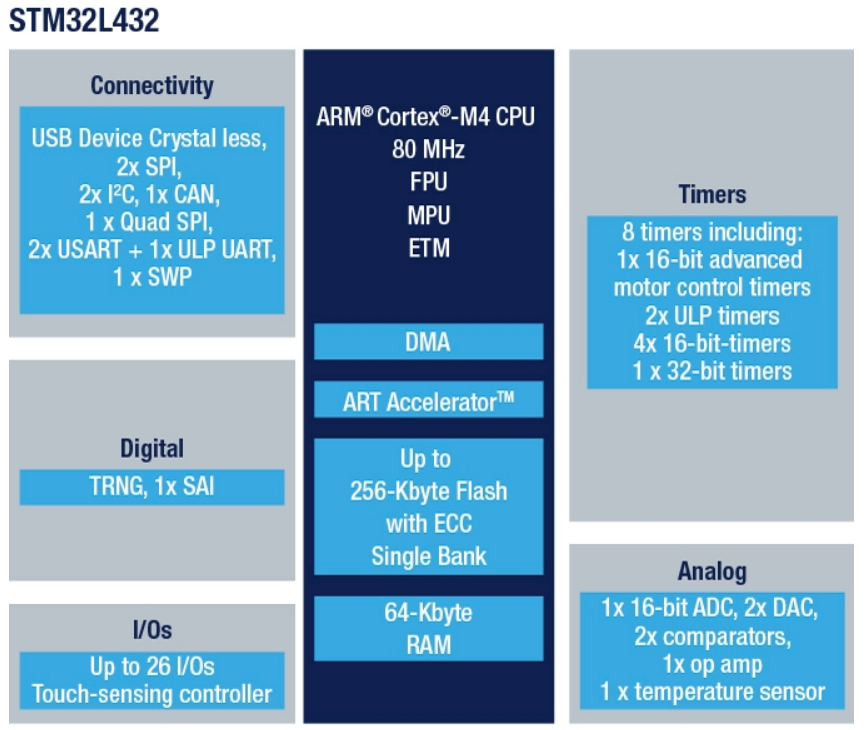
\includegraphics[width=0.8\textwidth]{./img/imagensExplicacoes/diagramaArm.png}
     \caption*{Fonte: ST.}
     \label{fig:diagArm}
\end{figure}


O kit foi escolhido por sua funcionalidade, preço, disponibilidade e facilidade de funcionamento. Todo o desenvolvimento do software necessário para a utilização do mesmo foi feito com o auxilio de uma ferramenta da empresa ST, o STM32Cube, que gera o código base para o funcionamento e configuração dos periféricos, e o TrueStudio - Atollic que é o editor de texto do programa, capaz de gravar e utilizar a depuração em hardware do kit.

O microcontrolador foi programado em C, utilizando bibliotecas HAL (Hardware Abstraction Layer) para facilitar e acelerar o desenvolvimento do firmware. As tarefas realizadas pelo microcontrolador foram implementadas na forma de uma máquina de estados que pode ser observada na figura \ref{fig:states}. As ações do microcontrolador dependem dos dados de comando recebidos serialmente. A tarefa de cada estado é explicada na tabela \ref{tab:states}.


\begin{figure}[H]
    \centering
     \caption{Kit de desenvolvimento STM32L432KCU6.}
     \includegraphics[width=0.4\textwidth]{./img/imagensExplicacoes/armkit.png}
     \caption*{Fonte: rs-online.}
     \label{fig:kitArm}
\end{figure}

\begin{table}[H]
    \centering
    \caption{Descrição dos estados.}
    \begin{tabular}{|p{4cm}|p{10cm}|}
     \hline
     \textbf{Simbolo do estado} & \textbf{Descrição do estado} \\
     \hline
     IDDLE & Estado que aguarda o recebimento de outro estado. \\ \hline
     I &  Define a polaridade para \textit{set} na ponte H conectada ao canal 2 e envia de volta `` `I' done!". \\ \hline
     i & Define a polaridade para \textit{set} na ponte H conectada ao canal 2 e envia de volta `` `i' done!". \\ \hline
     M & Define a polaridade para \textit{set} na ponte H conectada ao canal 3 e envia de volta `` `m' done!". \\ \hline
     m & Define a polaridade para \textit{set} na ponte H conectada ao canal 3 e envia de volta `` `M' done!". \\ \hline
     E & Define a polaridade para \textit{set} na ponte H conectada ao canal 1 e envia de volta `` `E' done!". \\ \hline
     e & Define a polaridade para \textit{set} na ponte H conectada ao canal 1 e envia de volta `` `e' done!". \\ \hline
     S & Coloca todas as polaridades em uma referência e envie de volta `` `S' done!". \\ \hline
     C & Executa procedimentos de medição contínuos e envie-os para a comunicação USB sem voltar ao estado IDDLE.\\ \hline 
     D & Executa apenas um procedimento de medição e envia o resultado dos dados para a comunicação pela USB retornando as estado IDDLE.\\ \hline
     
    \end{tabular}
    \label{tab:states}
\end{table}

As polaridades mencionadas na tabela \ref{tab:states}, \textit{set} e \textit{reset}, são nomes dados a polaridades opostas, ou seja, se \textit{set} for representado por estado lógico alto, \textit{reset} é representado pelo estado lógico baixo. Há um estado diferente para cada polaridade possível nas bobinas de Helmholtz. Além do estado S, utilizado para calibração e do estado C, utilizado no desenvolvimento das bobinas, há também um estado D, utilizado para requisitar, adquirir e processar as informações da indução magnética provenientes do sensor MMC3416 (Sensor que se comunica por protocolo I2C, seção 3.1.4). Dentro desse estado, o microcontrolador adquire os dados dos registradores do sensor, logo após tratamento, os envia para o computador.

A espera por comandos no estado IDDLE é realizada através de \textit{pooling}, que é um laço em software que espera por um evento, verificando constantemente o \textit{buffer} de entrada serial do microcontrolador para troca de estado.

\begin{figure}[H]
    \centering
     \caption{Diagrama da maquina de estados implementada no STM32L432KCU6.}
     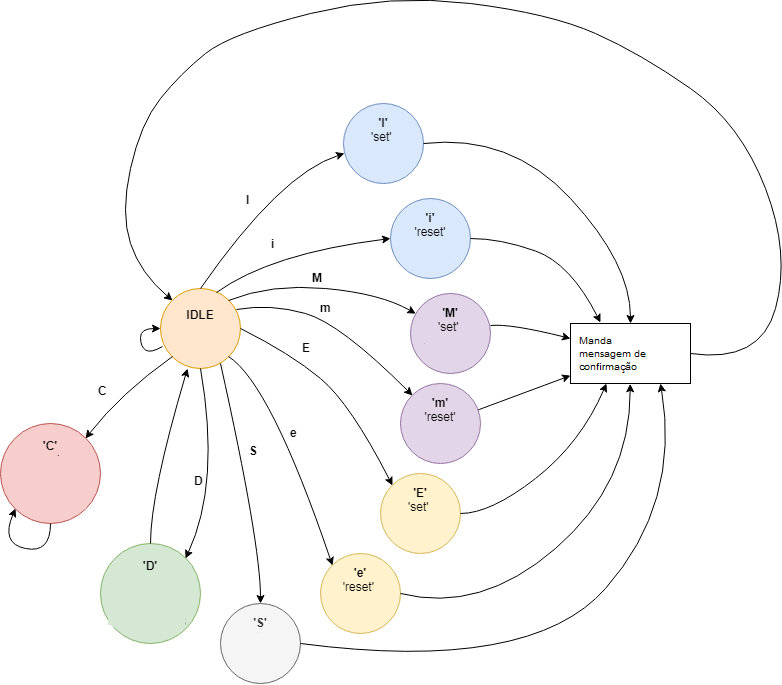
\includegraphics[width=0.8\textwidth]{./img/imagensExplicacoes/stateMachine.png}
     \caption*{Fonte: Autor.}
     \label{fig:states}
\end{figure}

\subsection{Sensor magnético}

O MMC3416 \cite{mcc3416} foi selecionado devido suas características de escala e resolução, mede em 3 direções, permitindo o ajuste de \textit{offset} pela utilização de uma função de \textit{set-reset} que anula o offset da medição \cite{AN213Ref}. É alimentado entre 1,8 e 3,6V e se comunica através do barramento I2C. Na figura \ref{fig:sensDiag} é apresentado o diagrama interno do componente.

\begin{figure}[H]
    \centering
     \caption{Diagrama interno do sensor.}
     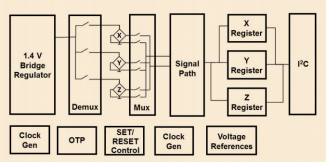
\includegraphics[width=0.8\textwidth]{./img/imagensExplicacoes/sensorDiag.png}
     \caption*{Fonte: Folha de dados do MMC3416.}
     \label{fig:sensDiag}
\end{figure}

A maior resolução possivelmente utilizada para este projeto seria de 1 $\mu$T. O MMC3416 tem resolução de 0.05 $\mu$T até 0.2 $\mu$T por \textit{bit} menos significativo, tendo uma escala com tamanho de 16 bits. Esse CI mede uma escala de $\pm$1600 $\mu$T, sendo este valor absolutamente maior que 1250 $\mu$T (Requisitos de geração da bobina). Além disso, o ruído \textit{RMS} (Ruído da raiz quadrada média) máximo é cerca de 0.15 $\mu$T, o que não acarreta erros significativos na medição.

Para rapidez no desenvolvimento empregou-se uma placa de avaliação na qual o sensor já vem montado. Essa placa é apresentada na figura \ref{fig:sensEval} e a mesma foi utilizada para o desenvolvimento do projeto.

\begin{figure}[H]
    \centering
     \caption{Hardware da placa de avaliação do sensor.}
     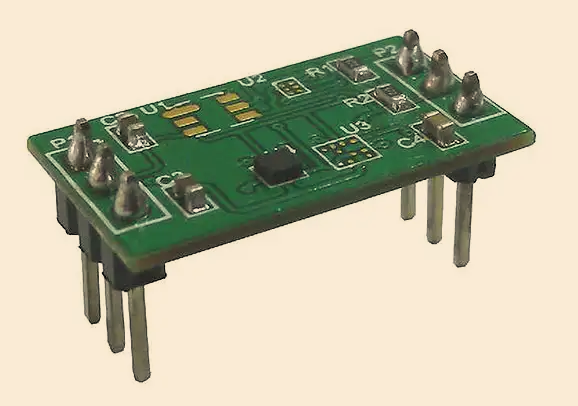
\includegraphics[width=0.6\textwidth]{./img/imagensExplicacoes/sensorEval.png}
     \caption*{Fonte: Folha de dados da placa de avaliação.}
     \label{fig:sensEval}
\end{figure}

\section{Placas de Circuito Impresso}

Mesmo utilizando uma placa de avaliação e um kit microcontrolado, era necessária a interligação entre essas placas em um único sistema. Assim, foram projetadas duas PCIs (Placas de Circuito Impresso)  empregando o software EAGLE (7.1) \cite{EagleWiki}. Uma PCI para receber o cabeamento necessário para o sensor e a outra, para conexão do kit microcontrolado com as demais partes do sistema. 

\subsection{PCI do sensor}

É a PCI mais simples, o sensor é centrado exatamente no meio da placa. Na figura \ref{fig:esqDesSens} é mostrado o esquemático e projeto do circuito. O circuito é uma simples ligação dos pinos do sensor até um conector do tipo KK \cite{KKcon}. Cada pino de sinal é acompanhado por um pino de referencia, sendo o cabo formado por pares levemente trançados para diminuir possíveis interferências no sinal.

\begin{figure}[H]
    \centering
     \caption{PCI do sensor}
     \subfloat[Esquemático]{%
       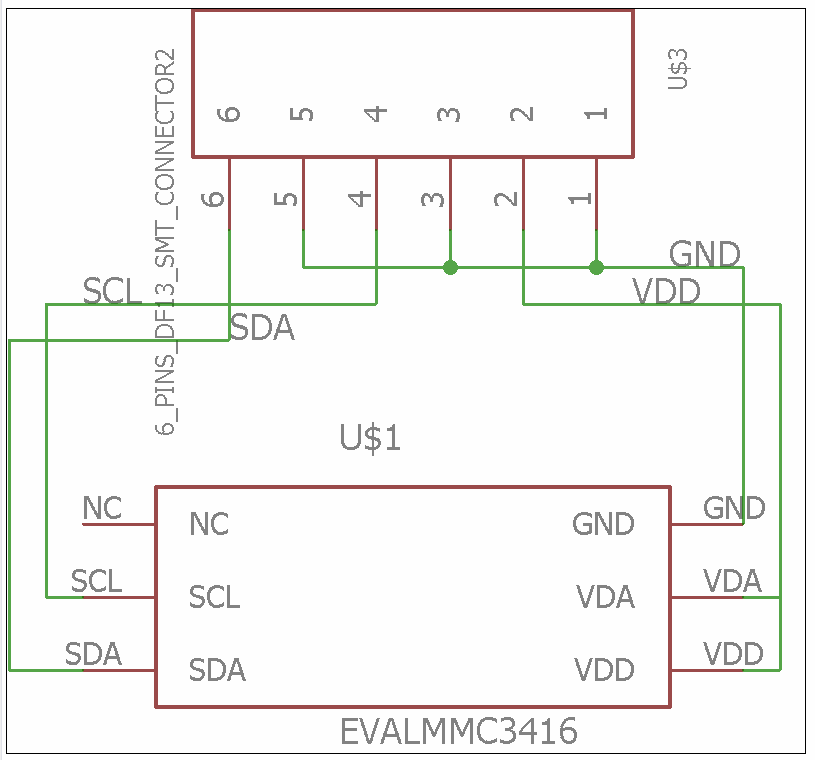
\includegraphics[width=0.35\textwidth]{./img/PCBs/esquematicoSensor.png}
     }
     \subfloat[Desenho de PCI]{%
       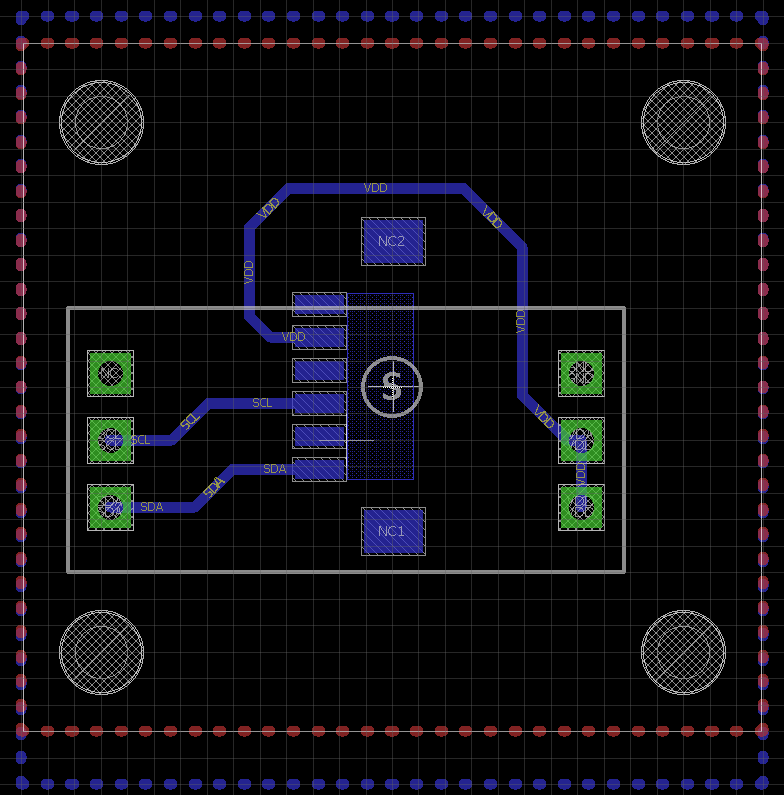
\includegraphics[width=0.35\textwidth]{./img/PCBs/desenhoSensor.png}
     }
    % \hfill
     \caption*{Fonte: Autor.}\label{fig:esqDesSens}
\end{figure}


\subsection{PCI do sistema}

A PCI do sistema une as bobinas de Helmholtz, o sensor, a fonte e o computador. Estão nela inseridos as pontes H, conectores para as bobinas, para o sensor e para a fonte. Também, permite o encaixe do kit STM32, que é conectado ao computador através do um cabo USB. A figura \ref{fig:esqMain} apresenta o esquemático dessa PCI.

\begin{figure}[H]
    \centering
     \caption{Esquemático da placa principal}
     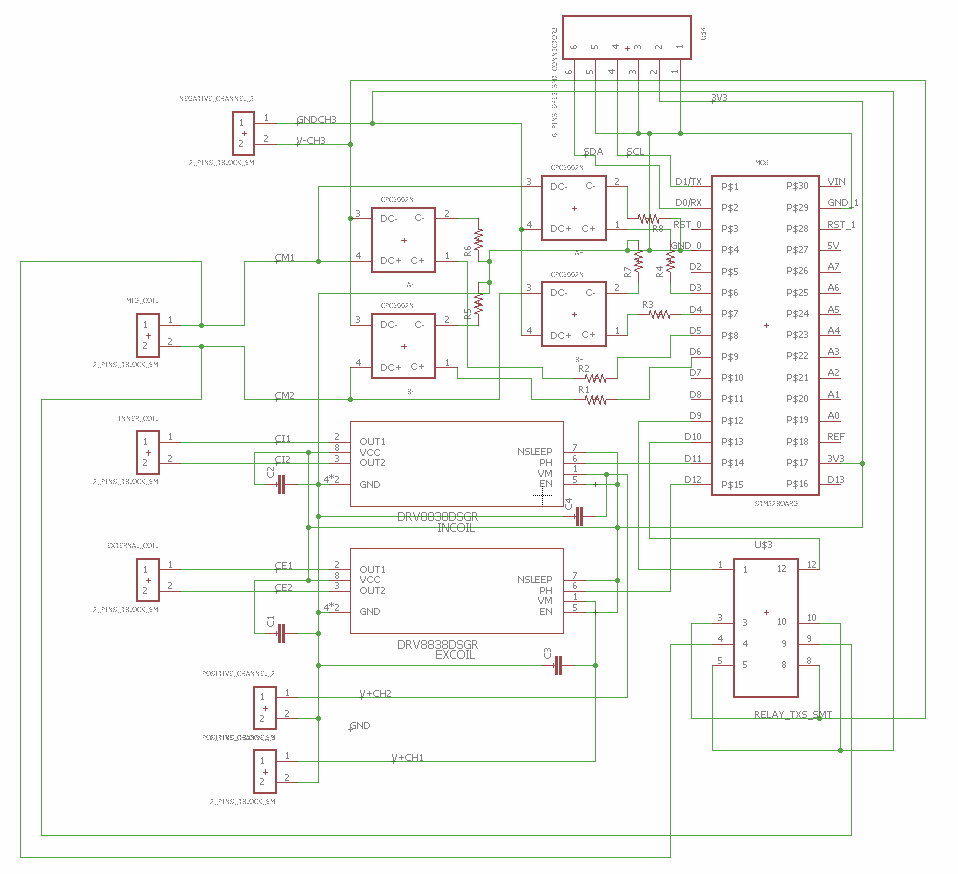
\includegraphics[width=1\textwidth]{./img/PCBs/esquematicoMain.png}
     \caption*{Fonte: Autor.}\label{fig:esqMain}
\end{figure}

No projeto da placa pode-se observar alguns furos metalizados (figura \ref{fig:desMain}), tendo trilhas tanto na parte superior quanto na inferior da PCI. Todos os componentes referentes às pontes H são SMDs. Na figura \ref{fig:pbcMain} é apresentado a PCI montada, todos os componentes foram inseridos manualmente, com colocação de pasta de solda utilizando um \textit{stencil}. Para a solda foi utilizado um forno elétrico doméstico.

\begin{figure}[H]
    \centering
     \caption{Desenho da PCI principal}
     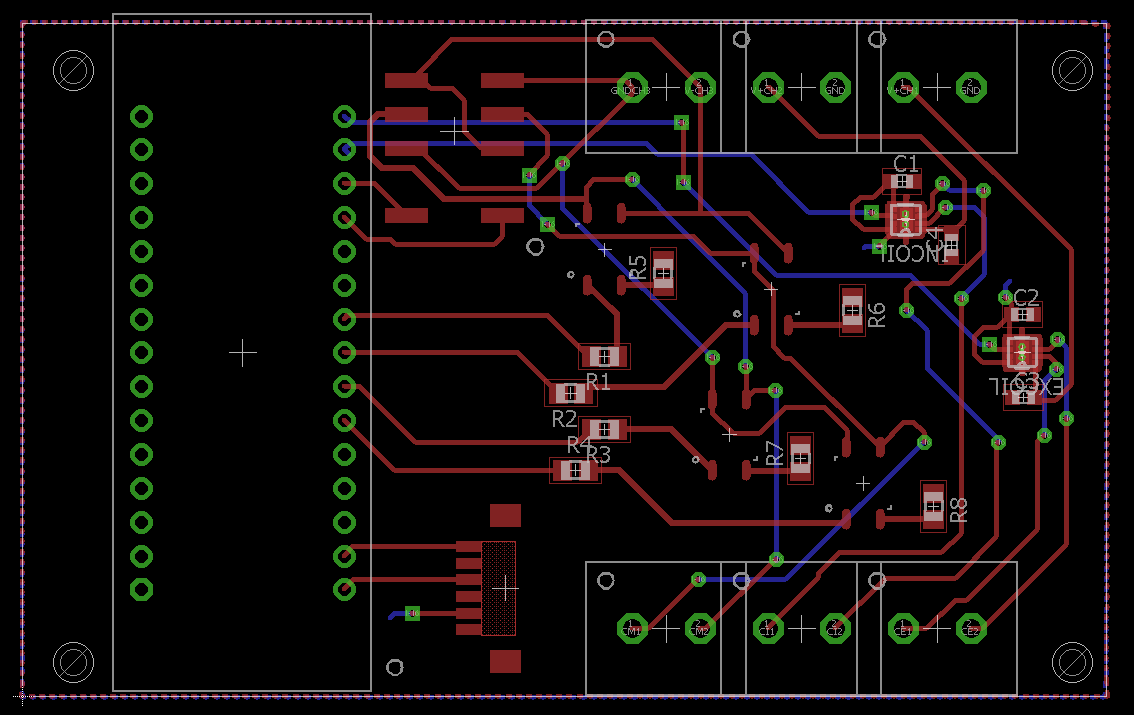
\includegraphics[width=0.55\textwidth]{./img/PCBs/desenhoMain.png}
     \caption*{Fonte: Autor.}\label{fig:desMain}
\end{figure}

\section{Bobinas de Helmholtz}

Para o auxílio no projeto das bobinas, tal como estimativa de formato e intensidade do campo, um simulador foi desenvolvido utilizando a magpylib \cite{magpy2020}.

Analisando-se os tamanhos de fios disponíveis, decidiu-se trabalhar com o AWG 23, utilizando a máxima corrente de 500 $mA$. Este valor de corrente não gerará potências maiores que 2 $W$, importante para o não derretimento das estruturas mecânicas de suporte das bobinas. Esse valor de corrente foi decidido após algumas iterações utilizando o simulador descrito na seção seguinte (3.3.1), através da resistência estimada das bobinas.

\subsection{Simulador}

Para simular as espiras nas posições corretas é necessário um modelo em função da geometria das bobinas de Helmholtz. Na modelagem, foi utilizada a secção de corte transversal dos enrolamentos, como mostrado na figura \ref{fig:cross}.

\begin{figure}[H]
    \centering
     \caption{Exemplo de seção transversal da bobina.}
     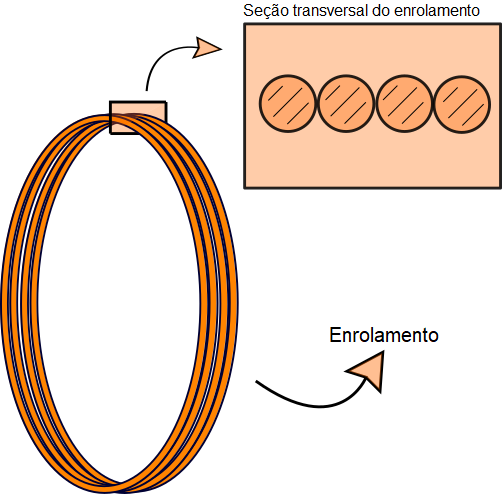
\includegraphics[width=0.5\textwidth]{./img/imagensExplicacoes/coil explanation.png}
     
     \caption*{Fonte: Autor.}\label{fig:cross}
\end{figure}

Os parâmetros para a modelagem da bobina estão sendo mostrados na figura \ref{fig:model}.

\begin{figure}[H]
    \centering
     \caption{Modelagem das bobinas}
     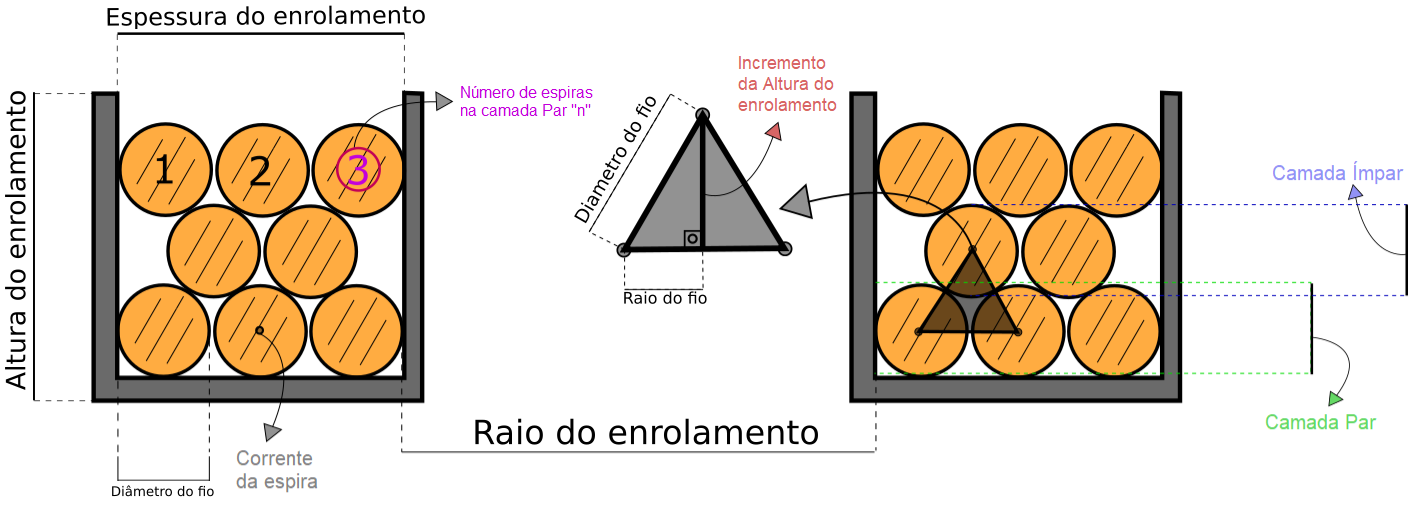
\includegraphics[width=1.05\textwidth]{./img/imagensExplicacoes/coil cross cut.png}
     
     \caption*{Fonte: Autor.}\label{fig:model}
\end{figure}

A partir do modelo das bobinas fez-se um programa em \textit{python} utilizando a \textit{magpylib}, capaz de calcular iterativamente o raio necessário para cada bobina, de forma a obter-se o campo desejado na região de interesse.

Além dos parâmetros do modelo, haviam outros parâmetros de entrada necessários para as iterações:

\begin{itemize}
    \item Número de laços nas camadas de laços Par.
    \item Número de camadas de laços Par e Ímpar.
    \item A indução desejada com a corrente máxima da bobina em $mT$.
    \item Corrente máxima da bobina em $mA$.
\end{itemize}

O modelo utiliza os parâmetros supracitados garantindo o funcionamento das bobinas da maneira esperada. Para facilitar a construção, ao invés do software utilizar o número de espiras de cada enrolamento, ele utiliza com o número de camadas pares e ímpares como parâmetro de entrada. No código a seguir é ilustrado o uso desses parâmetros para o cômputo do raio correto das bobinas.

%% Codigo
\inputminted[
frame=lines,
framesep=1mm,
baselinestretch=0.5,
fontsize=\footnotesize,
linenos
]{python}{codigos/sim.py}

O programa gera vários gráficos da geometria das bobinas e estima valores sobre parâmetros, tais como, comprimento de fio e potência dissipada.

Nos gráficos da figura \ref{fig:eixos} são mostrados o formato das 3 bobinas de Helmholtz em seus respectivos eixos. A bobina z tem mais enrolamentos que as outras pelo fato de ter uma especificação de campo maior. O que é visível nesses gráficos é que cada bobina foi dimensionada de forma ortogonal umas as outras, gerando 3 campos magnéticos em 3 direções linearmente independentes.

\begin{figure}[H]
    \centering
     \caption{Ilustração gráfica das bobinas}
     \subfloat[eixo 'z']{%
       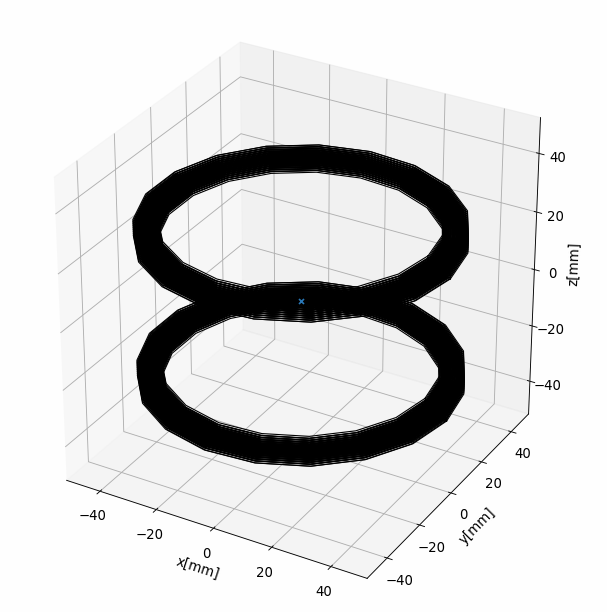
\includegraphics[width=0.3\textwidth]{./img/simulacao/zcoil.png}
     }
     \subfloat[eixo 'y']{%
       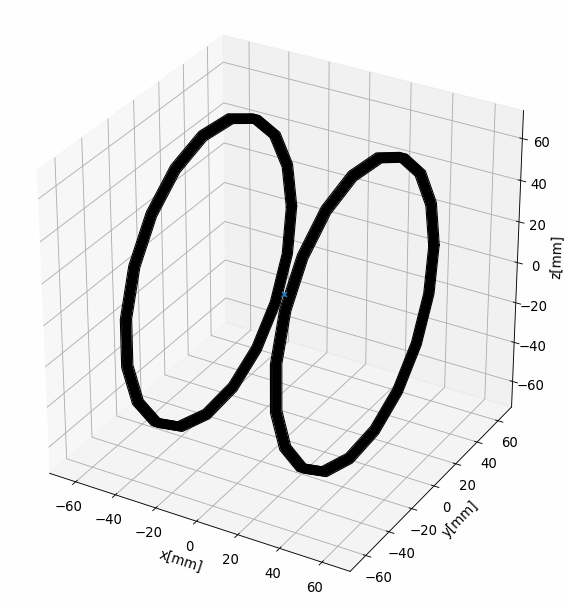
\includegraphics[width=0.3\textwidth]{./img/simulacao/ycoil.png}
     }
     \subfloat[eixo 'x']{%
       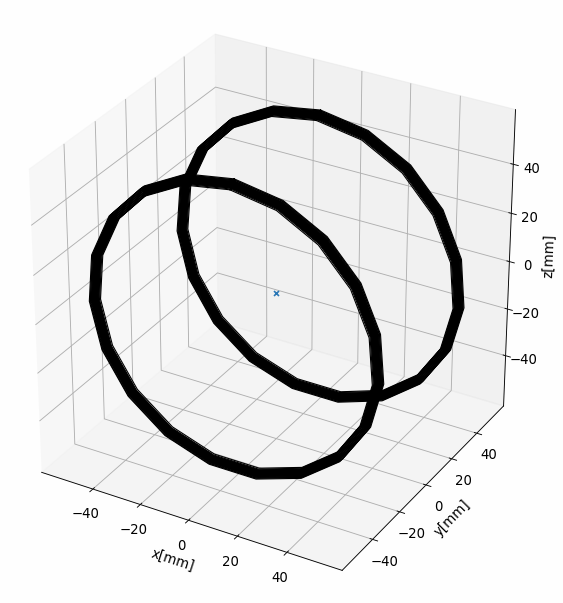
\includegraphics[width=0.3\textwidth]{./img/simulacao/xcoil.png}
     }
    % \hfill
     \caption*{Fonte: Autor.}\label{fig:eixos}
\end{figure}

Concomitante aos gráficos da figura \ref{fig:eixos}, são mostrados gráficos do campo magnético gerado na região de interesse. As figuras \ref{fig:grafz}, \ref{fig:grafy} e \ref{fig:grafx} demonstram curvas de nível em um plano de 20 mm x 20 mm no centro de cada uma das três estrutura. Exitem 4 gráficos em cada uma das 3 figuras supracitadas. Todos os 4 tem unidades de mm nos eixos horizontal e vertical. Em cada gráfico aparecem curvas de nível com seus respectivos valores, sendo as cores do gráfico uma ideia de potencial.

O gráfico superior esquerdo representa valores percentuais. Cada valor do gráfico é a diferença percentual de indução magnética do ponto em relação a indução magnética no centro da estrutura (0,0).

Nos demais gráficos, os valores das curvas de nível representam valores da indução magnética absoluta, todos dados em $\mu$T. O que difere os 3 gráficos é a direção vetorial do campo, sendo todos os pontos do gráfico superior direito na direção x, o inferior esquerdo na direção y e o inferior direito na direção z.

Os gráficos da figura \ref{fig:grafz} são relacionado com a bobina da figura \ref{fig:eixos} (a), sendo os gráficos das figuras \ref{fig:grafy} e \ref{fig:grafx} relacionados à figura \ref{fig:eixos} (b) e (c) respectivamente.
    
\begin{figure}[H]
    \centering
     \caption{Gráfico da indução magnética estimada na região de interesse (z)}
     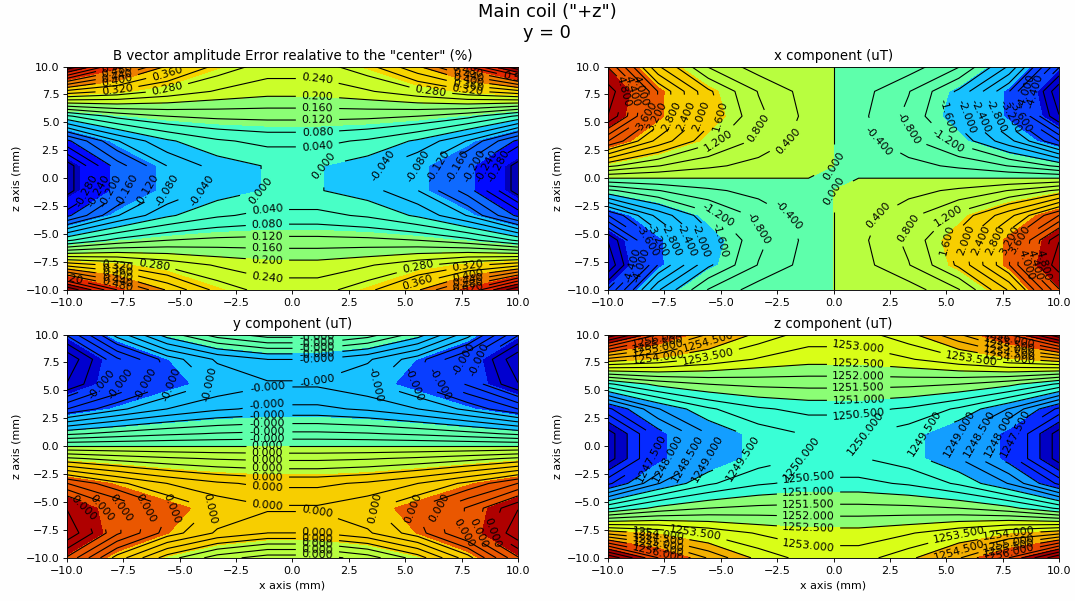
\includegraphics[width=1\textwidth]{./img/simulacao/mainCoilZ.png}
     \caption*{Fonte: Autor.}\label{fig:grafz}
\end{figure}


\begin{figure}[H]
    \centering
     \caption{Gráfico da indução magnética estimada na região de interesse (y)}
     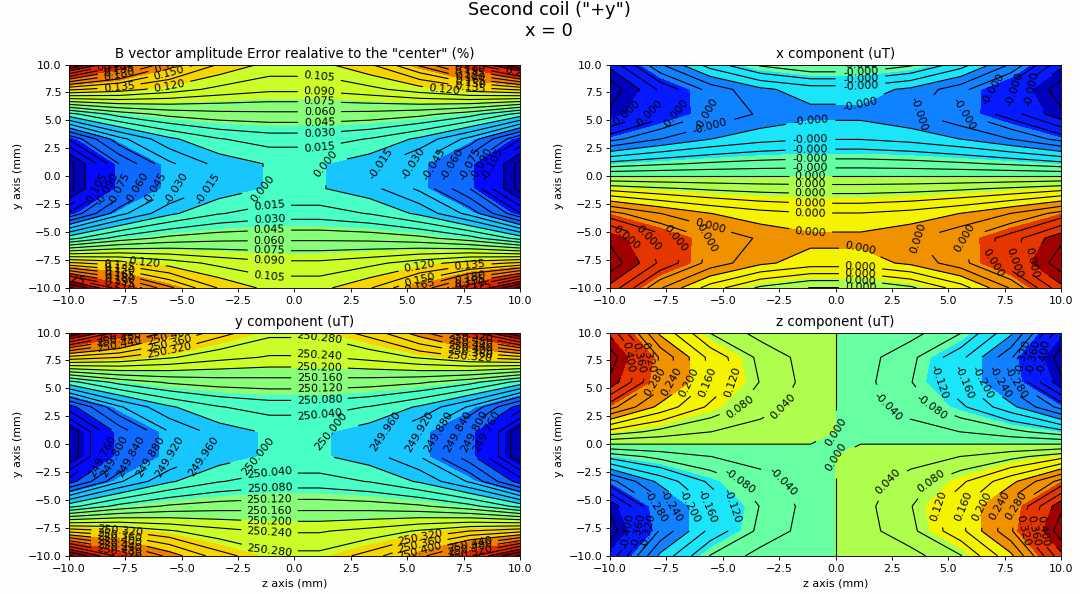
\includegraphics[width=1\textwidth]{./img/simulacao/secondCoily.png}
     \caption*{Fonte: Autor.}\label{fig:grafy}
\end{figure}

\begin{figure}[H]
    \centering
     \caption{Gráfico da indução magnética estimada na região de interesse (x)}
     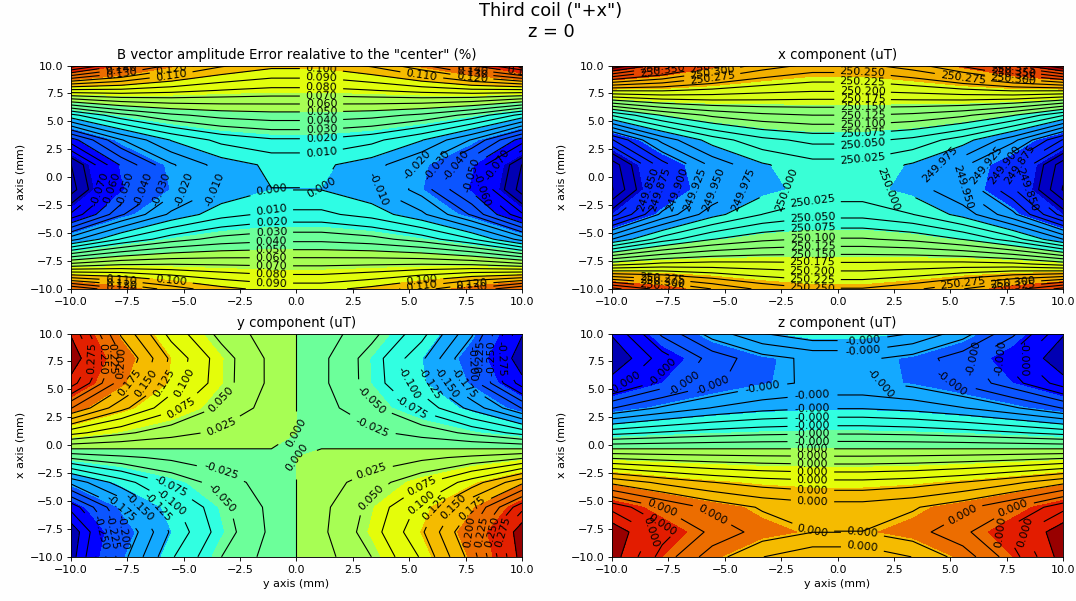
\includegraphics[width=1\textwidth]{./img/simulacao/thirdCoilx.png}
     \caption*{Fonte: Autor.}\label{fig:grafx}
\end{figure}

Há dois parâmetros a serem analisados com as figuras \ref{fig:grafz}, \ref{fig:grafy} e \ref{fig:grafx}: 

\begin{itemize}
    \item A diferença de intensidade da indução magnética gerada em cada ponto da região de interesse em relação a intensidade gerada no centro da bobina (0,0).
    \item A diferença de direção do campo gerado em cada ponto do gráfico em relação a direção do ponto central do gráfico.
\end{itemize}

Para notar a diferença de intensidade da indução magnética, basta observar o gráfico superior esquerdo das figuras anteriores. Se não houver nenhum valor maior que 1,  significa que em questão de módulo, a bobina cumpre com o requisito de homogeneidade de amplitude segundo objetivos. Para o cumprimento do requisito de direção de campo, o ângulo formado pelos vetores em cada ponto do gráfico não deve ser maior do que um grau em relação à direção de interesse de cada bobina.

Na verificação dessa diferença de direção é necessária a análise do ângulo formado em cada ponto do vetor em relação a direção desejada. Ou seja, na bobina com direção desejada em z, é necessária a análise do ângulo formado nos planos zy e zx. Se os ângulos dos vetores em relação a direção z forem menores do que um grau nos dois planos, então o requisito de homogeneidade de direção é cumprido.

Para a análise foram verificados nos gráficos os pontos de maiores amplitudes nos dois planos e na direção desejada. Nessa análise é realizado o cálculo da tangente do vetor utilizando o cateto oposto (outra direção) e o cateto adjacente (direção de interesse). O resultado do cálculo é comparado com a tangente de um grau. Se for menor, a bobina Helmholtz passa no teste e a região de interesse é considerada homogênea. Na equação \ref{eq:anghomo} é possível observar a relação entre a tangente de um grau e a tangente do vetor a ser analisado.

\begin{equation}
    \hspace{2pt}\textrm{tg}(1º) = 0.01745 \geq \frac{vetor_{outraDirecao}}{vetor_{DirecaoDeInteresse}}
    \label{eq:anghomo}
\end{equation}

O valor das tangentes nos dois planos, para o ponto com maior amplitude nas direções não desejadas em cada bobina Helmholtz é apresentado na figura \ref{fig:raz}. Pode-se observar que os valores encontrados foram até 5 vezes menores que o valor da tangente de um grau, validando o requisito de ângulo dos vetores na região de interesse segundo objetivos.

\begin{figure}[H]
    \centering
     \caption{Razões entre a direção não desejada e a direção desejada (código em python)}
     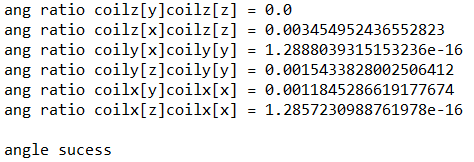
\includegraphics[width=0.8\textwidth]{./img/simulacao/angulo_console.png}
     \caption*{Fonte: Autor.}\label{fig:raz}
\end{figure}

Na figura \ref{fig:3dcoil} é possível observar que há espaço entre as bobinas, não havendo sobreposição de um enrolamento em outro, ou seja, quando a bobina for confeccionada, os enrolamentos terão distância radial suficiente para não colidirem fisicamente na hora que forem enrolados.

\begin{figure}[H]
    \centering
     \caption{Ilustração das 3 bobinas.}
     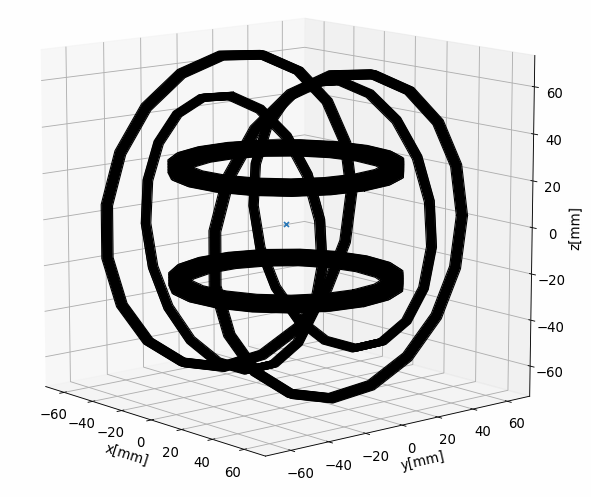
\includegraphics[width=0.65\textwidth]{./img/simulacao/desenhoCoil3D.png}
     \caption*{Fonte: Autor.}\label{fig:3dcoil}
\end{figure}

Na figura \ref{fig:cons} é possível observar as informações calculadas a partir dos parâmetros selecionados. Esses parâmetros serão utilizados no desenvolvimento e confecção do suporte mecânico das bobinas.

\begin{figure}[H]
    \centering
     \caption{Parâmetros calculados para a confecção do suporte mecânico das bobinas.}
     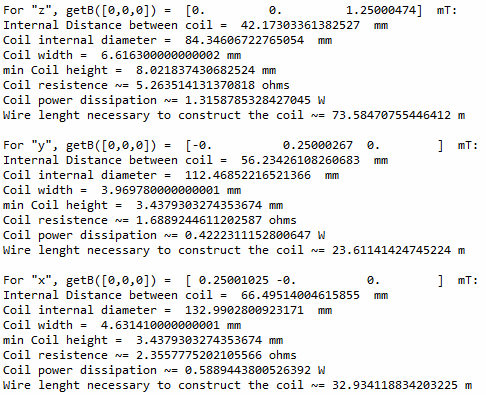
\includegraphics[width=0.67\textwidth]{./img/simulacao/console.png}
     \caption*{Fonte: Autor.}\label{fig:cons}
\end{figure}

As informações mostradas representam respectivamente para cada bobina:

\begin{itemize}
    \item O campo estimado no centro da estrutura em $mT$.
    \item A distância entre os dois enrolamentos de cada bobina de Helmholtz em mm.
    \item O diâmetro interno dos enrolamentos de cada bobina de Helmholtz em mm.
    \item A espessura do enrolamento (Citado na figura \ref{fig:model}) da bobina de Helmholtz em mm.
    \item A altura do enrolamento (Citado na figura \ref{fig:model}) da bobina de Helmholtz em mm.
    \item A resistência estimada para cada bobina de Helmholtz em $\Omega$.
    \item A potência dissipada por cada bobina de Helmholtz em W.
    \item A quantidade de fio em metros necessária para construir cada bobina.
\end{itemize}

Na tabela \ref{tab:paramSim} são listados os parâmetros calculados para o desenvolvimento do suporte dos enrolamentos das bobinas de Helmholtz, raio dos enrolamentos de cada bobina, espessura do enrolamento e altura do enrolamento de cada bobina de Helmholtz.

\begin{table}[H]
    \centering
    \caption{Parâmetros retirados do simulador}
    \begin{tabular}{ |p{2.5cm}|p{2cm}|p{3.9cm}|p{4.4cm}|}
     \hline
     \textbf{Bobina} & \textbf{Raio} & \textbf{Espessura vertical}& \textbf{Espessura horizontal} \\
     \hline
     Interna & 42.5 mm & 6.6 mm & 9.65 mm \\
     Intermediária & 56.15 mm & 4 mm & 5.5 mm \\
     Externa & 66.5 mm & 4.65 mm & 5.5 mm \\
     \hline
    \end{tabular}
    \label{tab:paramSim}
\end{table}


\subsection{Modelos 3D}

Para evitar problemas de desalinhamento e de montagem mecânica optou-se pela confecção de uma peça única, onde as três bobinas seriam enroladas.

O modelo para o suporte das bobinas é mostrado na figura \ref{fig:mod3D}, desenhado no software solidWorks \cite{solidWorks}. Nesse modelo é possível observar cinco orifícios na visão superior. Quatro desses orifícios serão utilizados para a fixação do suporte do sensor do sistema e o transdutor a ser avaliado, sendo o orifício central utilizado para a passagem de fios de conexão com os sensores.


\begin{figure}[H]
    \centering
     \caption{Modelo do suporte das bobinas.}
     \subfloat[Visão lateral.]{%
       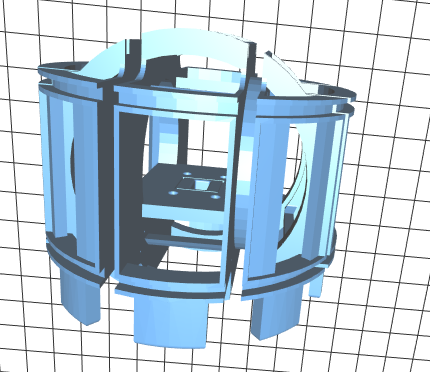
\includegraphics[width=0.3\textwidth]{./img/modelos3D/3DHC model.png}
     }
     \subfloat[Visão inferior.]{%
       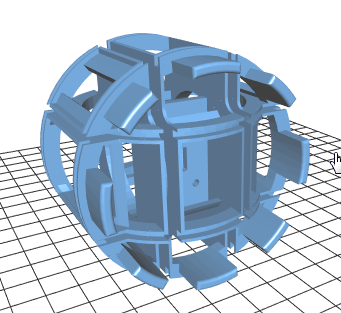
\includegraphics[width=0.3\textwidth]{./img/modelos3D/3DHC model 2.png}
     }
     \subfloat[Visão superior.]{%
       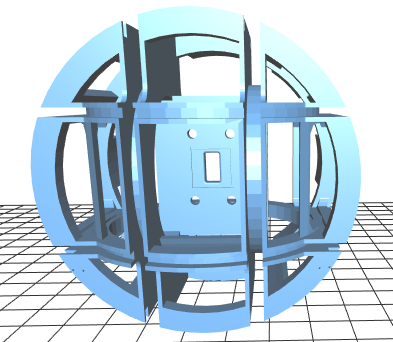
\includegraphics[width=0.3\textwidth]{./img/modelos3D/3DHC model 3.png}
     }
    % \hfill
     \caption*{Fonte: Autor.}\label{fig:mod3D}
\end{figure}

A seguir o modelo do suporte do sensor do sistema e do transdutor produzido pela SAL. O modelo pode ser visto na figura \ref{fig:sups}, sendo os quatro pilares centrais o suporte do sensor do sistema e a estrutura planar mais externa o suporte do transdutor a ser avaliado.

\begin{figure}[H]
    \centering
     \caption{Modelo do suporte do sensor.}
     \subfloat[Visão superior]{%
        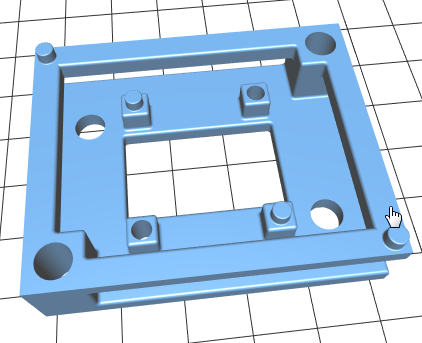
\includegraphics[width=0.5\textwidth]{./img/modelos3D/sensor support.png}
     }
     \subfloat[Visão inferior]{%
        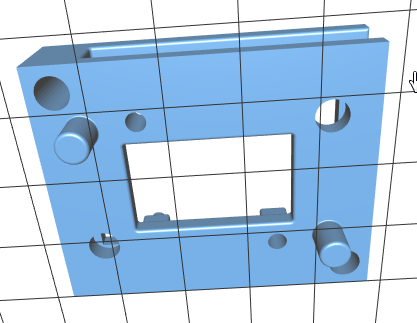
\includegraphics[width=0.5\textwidth]{./img/modelos3D/sensor support 2.png}
     }
    % \hfill
     \caption*{Fonte: Autor.}\label{fig:sups}
\end{figure}

Para a fixação do suporte do sensor foram confeccionados rebites de diversos tamanhos, que possibilitavam diferentes pressões para fixar o suporte do sensor e transdutor no suporte das bobinas. O modelo dos rebites pode ser observado na figura \ref{fig:reb}.

\begin{figure}[H]
    \centering
     \caption{Modelo dos rebites.}
     \subfloat[Visão inferior]{%
        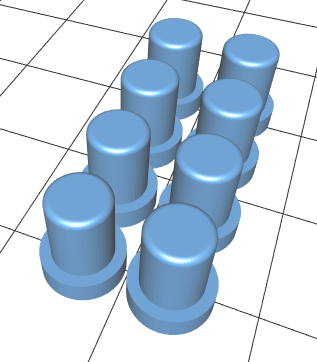
\includegraphics[width=0.32\textwidth]{./img/modelos3D/pegs example 1.png}
     }
     \subfloat[Visão superior]{%
        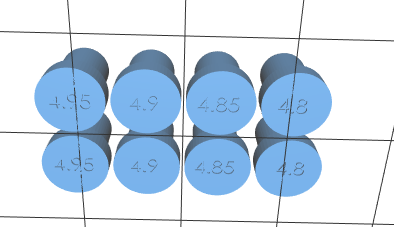
\includegraphics[width=0.68\textwidth]{./img/modelos3D/pegs example 2.png}
     }
    % \hfill
     \caption*{Fonte: Autor.}\label{fig:reb}
\end{figure}

Para uma menor interação das bobinas com possíveis estruturas metálicas onde a bobina seria apoiada foi desenvolvido o modelo de um tripé que possa suportar as bobinas a uma altura equivalente a 20 cm, valor definido pelo orientador do projeto na empresa. O modelo deste tripé pode ser observado na figura \ref{fig:trip}.

\begin{figure}[H]
    \centering
     \caption{Modelo do tripé.}
     \subfloat[]{%
        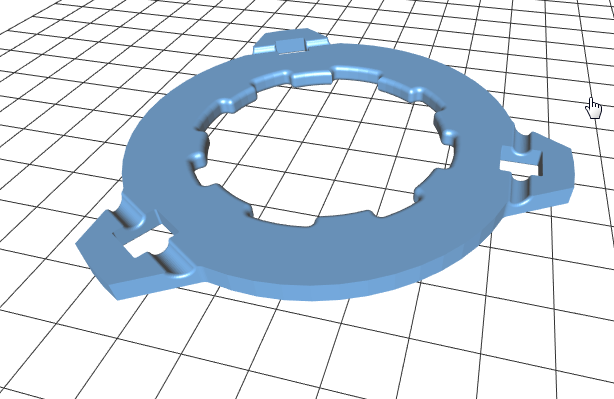
\includegraphics[width=0.4\textwidth]{./img/modelos3D/coils support 1.png}
     }
     \subfloat[]{%
        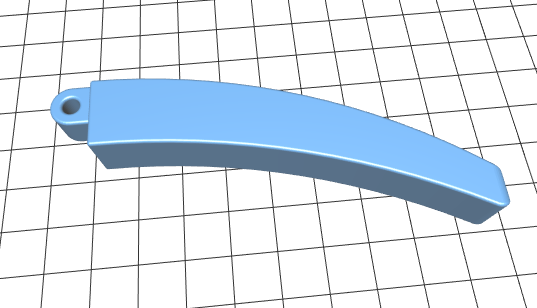
\includegraphics[width=0.4\textwidth]{./img/modelos3D/coil support 2.png}
     }
     \subfloat[]{%
        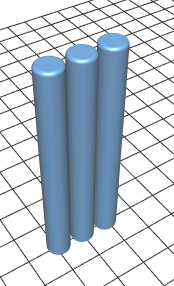
\includegraphics[width=0.15\textwidth]{./img/modelos3D/coil support 3.png}
     }
    % \hfill
     \caption*{Fonte: Autor.}\label{fig:trip}
\end{figure}

\section{Processamento de dados}

\subsection{Matriz de rotação}

É inerente da medição o desalinhamento entre a direção do campo gerado pelas bobinas e a direção de indução magnética medida pelo sensor, pois o mesmo estará de alguma forma com seu eixos de medição deslocados dos eixos do campo gerado. Para resolver esse desalinhamento foi desenvolvida uma matriz de rotação que alinha o campo medido pelo sensor. A seguir é descrita a matriz de rotação, o cálculo em \textit{python} pode ser visto no apêndice A.

As informações conhecidas a respeito da geração dos campos magnéticos e da medição é:
\begin{itemize}
    \item Corrente elétrica injetada nas bobinas de Helmholtz, $I$.
    \item Valor de campo de indução magnética gerado apenas pelas bobinas de Helmholtz medido com o sensor no centro da estrutura, este chamado de $M$. 
    \item Razão entre corrente injetada e campo de indução magnética produzida por cada bobina, chamada de $Cb$.
\end{itemize}

Na equação \ref{eq:rot} é apresentada a relação entre as medidas obtidas e as medidas geradas após a transformação de rotação. Assumindo que $M$ está desalinhado em relação ao campo gerado por $I$ e representa a medida desse mesmo campo. A relação entre as matrizes $I$ e $M$, sem modificação da norma será chamada de $\mu$. A matriz $Cb$ é uma matriz que transforma as correntes $I$ em um valor correspondente de indução magnética, isso é feito através do produto interno entre $Cb$ e $I$.

\begin{gather}
\label{eq:rot}
 \begin{bmatrix} I\cdot C_b \end{bmatrix}_{3x1}
 =
  \begin{bmatrix}
   \mu
   \end{bmatrix}_{3x3}
 \begin{bmatrix} M \end{bmatrix}_{3x1}
\end{gather}

Sendo:

\begin{gather}
\label{eq:mI}
 \begin{bmatrix} I \end{bmatrix}_{3x1}
 =
  \begin{bmatrix}
   I_x \\
   I_y \\
   I_z
   \end{bmatrix}
\end{gather}


\begin{gather}
\label{eq:mM}
 \begin{bmatrix} M \end{bmatrix}_{3x1}
 =
  \begin{bmatrix}
   M_{xb} - M_{xa} \\
   M_{yb} - M_{ya} \\
   M_{zb} - M_{za}
   \end{bmatrix}
 =
  \begin{bmatrix}
   M_x \\
   M_y \\
   M_z
   \end{bmatrix}
\end{gather}

\begin{gather}
\label{eq:mC}
 \begin{bmatrix} C_b \end{bmatrix}_{3x1}
 =
  \begin{bmatrix}
   C_{bx} \\
   C_{by} \\
   C_{bz}
   \end{bmatrix}
\end{gather}

\begin{gather}
\label{eq:mu}
 \begin{bmatrix} \mu \end{bmatrix}_{3x3}
 =
  \begin{bmatrix}
   \mu_{x1} & \mu_{y1} & \mu_{z1} \\
   \mu_{x2} & \mu_{y2} & \mu_{z2} \\
   \mu_{x3} & \mu_{y3} & \mu_{z3} \\
   \end{bmatrix}
\end{gather}

Como o objetivo é lidar apenas com o campo gerado pelas bobinas, é feito primeiramente a medição do campo do ambiente, sem nenhuma bobina ligada, este chamado de $M_a$, outra medida $M_b$ com as bobinas ligadas. A subtração dessas duas medidas leva a medição do campo gerado apenas pelas bobinas.

Há nove incógnitas e apenas um direção linearmente independente. Todavia isto pode ser resolvido obtendo-se três medidas em três direções independentes. Obtendo-se três vezes mais informação é possível a resolução do sistema. Nas equações \ref{eq:rotA} e \ref{eq:rotB} é possível observar o sistema formado por essas três medições.

\begin{gather}
\label{eq:rotA}
 \begin{bmatrix} I_1\cdot C_{b}  & I_2\cdot C_{b}  & I_3\cdot C_{b}  \end{bmatrix}_{3x3}
 =
  \begin{bmatrix}
   \mu
   \end{bmatrix}_{3x3}
 \begin{bmatrix} M_1& M_2 & M_3 \end{bmatrix}_{3x3}
\end{gather}


\begin{gather}
\label{eq:rotB}
 \begin{bmatrix} I_{1x}\cdot C_{bx} & I_{2x}\cdot C_{bx} & I_{3x}\cdot C_{bx} \\
 I_{1y}\cdot C_{by} & I_{2y}\cdot C_{by} & I_{3y}\cdot C_{by} \\
 I_{1z}\cdot C_{bz} & I_{2z}\cdot C_{bz} & I_{3z}\cdot C_{bz} \\
 \end{bmatrix}
 =
   \begin{bmatrix}
   \mu_{x1} & \mu_{y1} & \mu_{z1} \\
   \mu_{x2} & \mu_{y2} & \mu_{z3} \\
   \mu_{x3} & \mu_{y2} & \mu_{z3} \\
   \end{bmatrix}
    \begin{bmatrix}
   M_{1x} & M_{2x} & M_{3x} \\
   M_{1y} & M_{2y} & M_{3y} \\
   M_{1z} & M_{2z} & M_{3z} \\
   \end{bmatrix}
\end{gather}

$Cb$ é a razão entre o campo gerado pela bobina e a corrente na mesma. Essa matriz pode ser encontrado através de um procedimento simples:

\begin{itemize}
    \item Mede-se o campo no centro da bobina, sabendo que este é o campo atual naquele ponto, chamando a medida de $M_{cb1}$
    \item Aplica-se uma corrente $I_{cb}$ conhecida na bobina e mede-se o campo no centro da bobina outra vez, sem movimentar o sensor de lugar, chamando esta medida de $M_{cb2}$
\end{itemize}

A intensidade do campo gerado $Cg$ pela bobina será exatamente a norma da diferença entre $M_{cb2}$ e $M_{cb1}$. Sabendo a corrente $I_{cb}$ é possível determinar-se $Cb$ fazendo a razão entre $Cg$ e $I_{cb}$, o que pode ser observado na equação \ref{eq:cbfrac}.

\begin{equation}
    \label{eq:cbfrac}
    C_b = \frac{C_g}{I_{cb}}
\end{equation}

Sendo conhecidas as matrizes $I$, $M$ e $Cb$ é possível determinar $\mu$ através da resolução do sistema linear. O código de cálculo da chamada matriz de rotação $\mu$ pode ser observado no apêndice A.

\subsection{Aumento da relação Sinal Ruído através de média}

O ruído RMS do sensor utilizado é de 0.15 $\mu$T \cite{mcc3416}. Essa característica pode ser melhorada através de média, dado que os campos gerados devem permanecer estáticos do começo ao fim da medida. A equação \ref{eq:SRNn1} \cite{noiseRedArt} descreve o aumento da relação sinal ruído de uma média de medidas com número N ($SRN_N$) em relação a apenas uma medida ($SRN_1$).

\begin{equation}
    \label{eq:SRNn1}
    SRN_N = \sqrt{N}\cdot SRN_1
\end{equation}

Foi feito um teste empírico para observar qual seria o melhor valor de medidas N sem que ocorresse degradação do funcionamento do equipamento.

Sendo 1 $\mu$T o valor da resolução de sinal, na equação \ref{eq:SRN1}, é possível observar a relação sinal ruído para apenas uma amostra do sensor MMC3416. Esse valor é utilizado para o cálculo da relação sinal ruído com 30 amostras na equação \ref{eq:SRNN}. Há um ganho na SRN da medida de 6,66 para 36,5.


\begin{equation}
    \label{eq:SRN1}
    SRN_1 = \frac{1}{0.15} = 6.666
\end{equation}

\begin{equation}
    \label{eq:SRNN}
    SRN_N = \sqrt{30}\cdot 6.666 = 36.5
\end{equation}

Utilizando a nova relação sinal ruído encontrada, é possível calcular-se o novo ruído RMS de cada medida, o que pode ser observado na equação \ref{eq:RMSn}. O valor encontrado de 0,027 μT é 5,55 vezes menor que o valor anteriormente citado. Assim, se obtém um ganho de exatidão das medidas sem a degradação do desempenho do equipamento.

\begin{equation}
    \label{eq:RMSn}
    RMS_{noise} = \frac{1}{36.5} = 0.027 \mu T
\end{equation}